\documentclass{article}\usepackage[]{graphicx}\usepackage[]{color}
%% maxwidth is the original width if it is less than linewidth
%% otherwise use linewidth (to make sure the graphics do not exceed the margin)
\makeatletter
\def\maxwidth{ %
  \ifdim\Gin@nat@width>\linewidth
    \linewidth
  \else
    \Gin@nat@width
  \fi
}
\makeatother

\definecolor{fgcolor}{rgb}{0.345, 0.345, 0.345}
\newcommand{\hlnum}[1]{\textcolor[rgb]{0.686,0.059,0.569}{#1}}%
\newcommand{\hlstr}[1]{\textcolor[rgb]{0.192,0.494,0.8}{#1}}%
\newcommand{\hlcom}[1]{\textcolor[rgb]{0.678,0.584,0.686}{\textit{#1}}}%
\newcommand{\hlopt}[1]{\textcolor[rgb]{0,0,0}{#1}}%
\newcommand{\hlstd}[1]{\textcolor[rgb]{0.345,0.345,0.345}{#1}}%
\newcommand{\hlkwa}[1]{\textcolor[rgb]{0.161,0.373,0.58}{\textbf{#1}}}%
\newcommand{\hlkwb}[1]{\textcolor[rgb]{0.69,0.353,0.396}{#1}}%
\newcommand{\hlkwc}[1]{\textcolor[rgb]{0.333,0.667,0.333}{#1}}%
\newcommand{\hlkwd}[1]{\textcolor[rgb]{0.737,0.353,0.396}{\textbf{#1}}}%

\usepackage{framed}
\makeatletter
\newenvironment{kframe}{%
 \def\at@end@of@kframe{}%
 \ifinner\ifhmode%
  \def\at@end@of@kframe{\end{minipage}}%
  \begin{minipage}{\columnwidth}%
 \fi\fi%
 \def\FrameCommand##1{\hskip\@totalleftmargin \hskip-\fboxsep
 \colorbox{shadecolor}{##1}\hskip-\fboxsep
     % There is no \\@totalrightmargin, so:
     \hskip-\linewidth \hskip-\@totalleftmargin \hskip\columnwidth}%
 \MakeFramed {\advance\hsize-\width
   \@totalleftmargin\z@ \linewidth\hsize
   \@setminipage}}%
 {\par\unskip\endMakeFramed%
 \at@end@of@kframe}
\makeatother

\definecolor{shadecolor}{rgb}{.97, .97, .97}
\definecolor{messagecolor}{rgb}{0, 0, 0}
\definecolor{warningcolor}{rgb}{1, 0, 1}
\definecolor{errorcolor}{rgb}{1, 0, 0}
\newenvironment{knitrout}{}{} % an empty environment to be redefined in TeX

\usepackage{alltt}

\usepackage{amsmath, amssymb}
\IfFileExists{upquote.sty}{\usepackage{upquote}}{}
\begin{document}

\begin{knitrout}
\definecolor{shadecolor}{rgb}{0.969, 0.969, 0.969}\color{fgcolor}\begin{kframe}
\begin{alltt}
\hlkwd{rm}\hlstd{(}\hlkwc{list} \hlstd{=} \hlkwd{ls}\hlstd{())}
\hlkwd{library}\hlstd{(Zelig)}
\hlkwd{library}\hlstd{(arm)}
\hlkwd{data}\hlstd{(mid)}
\end{alltt}
\end{kframe}
\end{knitrout}

\section{Probit model of conflict}

\begin{knitrout}
\definecolor{shadecolor}{rgb}{0.969, 0.969, 0.969}\color{fgcolor}\begin{kframe}
\begin{alltt}
\hlstd{m_1} \hlkwb{<-} \hlkwd{glm}\hlstd{(conflict} \hlopt{~} \hlstd{major} \hlopt{+} \hlstd{contig} \hlopt{+} \hlstd{power} \hlopt{+} \hlstd{years,} \hlkwc{data} \hlstd{= mid,}
           \hlkwc{family} \hlstd{=} \hlkwd{binomial}\hlstd{(}\hlkwc{link} \hlstd{=} \hlstr{"probit"}\hlstd{))}
\end{alltt}
\end{kframe}
\end{knitrout}

\subsection{binnedplot of residuals against powers and years}

\begin{knitrout}
\definecolor{shadecolor}{rgb}{0.969, 0.969, 0.969}\color{fgcolor}\begin{kframe}
\begin{alltt}
\hlkwd{par}\hlstd{(}\hlkwc{mfrow} \hlstd{=} \hlkwd{c}\hlstd{(}\hlnum{2}\hlstd{,} \hlnum{1}\hlstd{))}
\hlkwd{binnedplot}\hlstd{(m_1}\hlopt{$}\hlstd{data}\hlopt{$}\hlstd{power,} \hlkwd{residuals}\hlstd{(m_1),} \hlkwc{xlab} \hlstd{=} \hlstr{"Power"}\hlstd{)}
\hlkwd{binnedplot}\hlstd{(m_1}\hlopt{$}\hlstd{data}\hlopt{$}\hlstd{year,} \hlkwd{residuals}\hlstd{(m_1),} \hlkwc{xlab} \hlstd{=} \hlstr{"Year"}\hlstd{)}
\end{alltt}
\end{kframe}
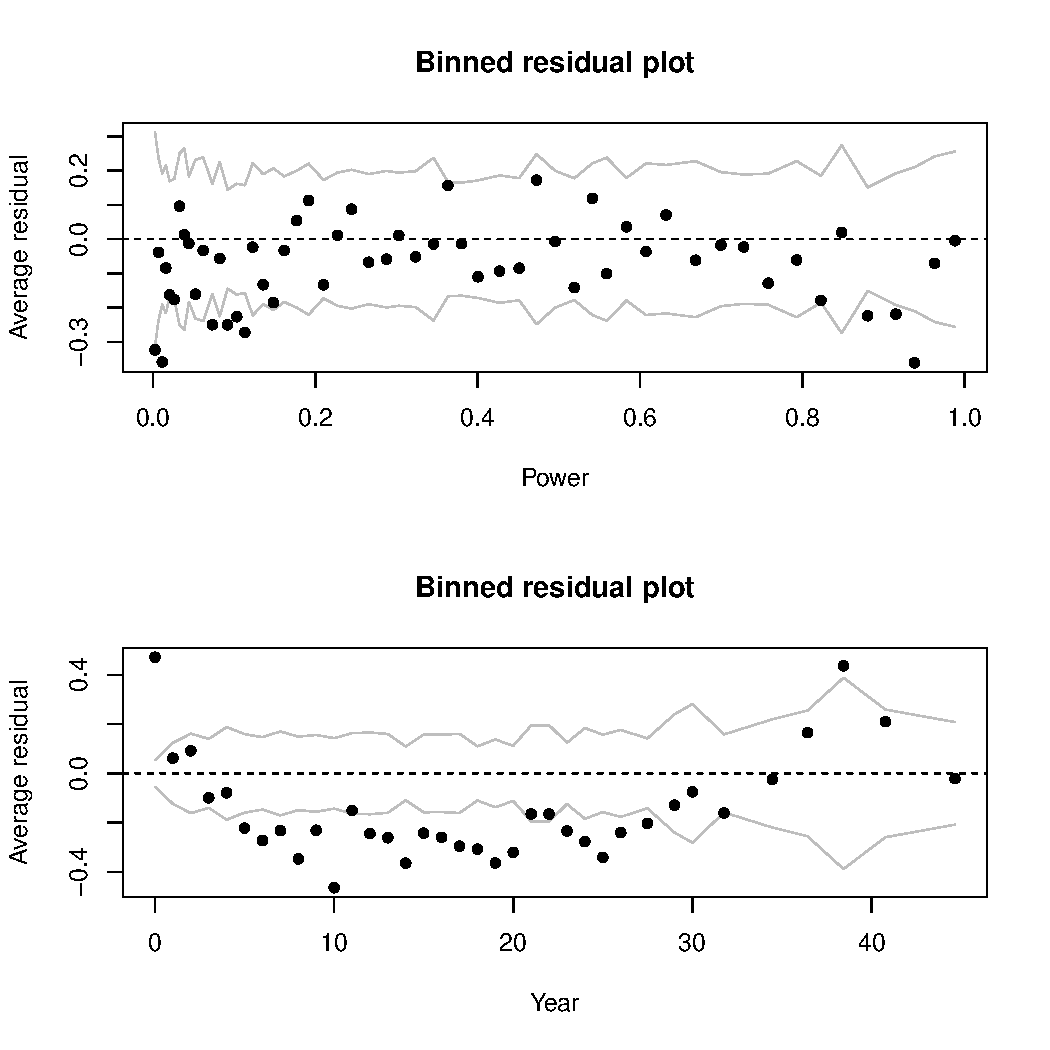
\includegraphics[width=\maxwidth]{figure/unnamed-chunk-2-1} 
\begin{kframe}\begin{alltt}
\hlkwd{par}\hlstd{(}\hlkwc{mfrow} \hlstd{=} \hlkwd{c}\hlstd{(}\hlnum{1}\hlstd{,} \hlnum{1}\hlstd{))}
\end{alltt}
\end{kframe}
\end{knitrout}

The fit looks pretty good especially for power (all residuals hover around 0). For year, the residuals seem to have a quadratic relationship and also big residuals near the two extremes of the distribution.

\subsection{Influence statistics to find problematic data point}

\begin{knitrout}
\definecolor{shadecolor}{rgb}{0.969, 0.969, 0.969}\color{fgcolor}\begin{kframe}
\begin{alltt}
\hlkwd{library}\hlstd{(car)}
\end{alltt}


{\ttfamily\noindent\itshape\color{messagecolor}{\#\# \\\#\# Attaching package: 'car'}}

{\ttfamily\noindent\itshape\color{messagecolor}{\#\# The following object is masked from 'package:arm':\\\#\# \\\#\#\ \ \ \  logit}}\begin{alltt}
\hlkwd{influenceIndexPlot}\hlstd{(m_1,} \hlkwc{vars}\hlstd{=}\hlkwd{c}\hlstd{(}\hlstr{"Cook"}\hlstd{,}\hlstr{"hat"}\hlstd{,}\hlstr{"Studentized"}\hlstd{),} \hlkwc{id.n}\hlstd{=}\hlnum{3}\hlstd{)}
\end{alltt}
\end{kframe}
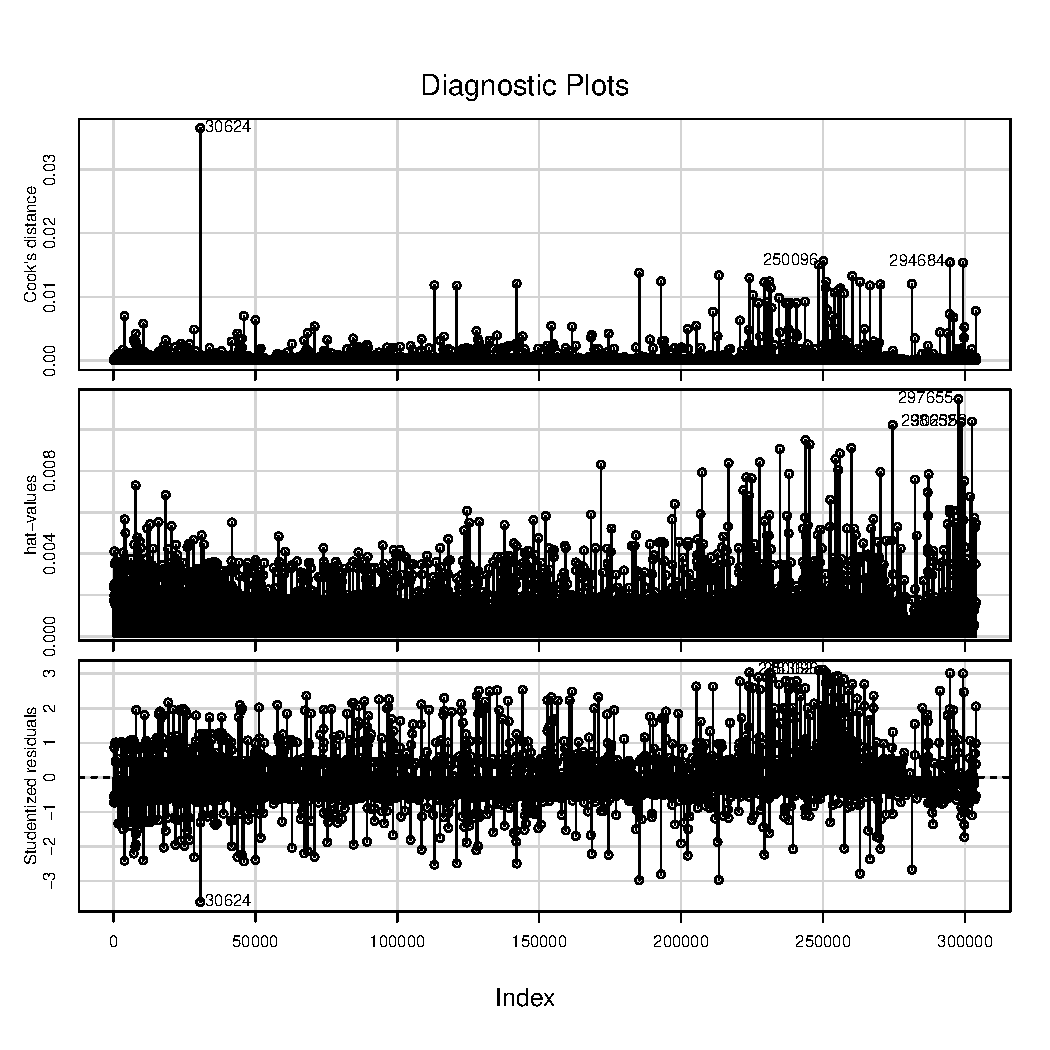
\includegraphics[width=\maxwidth]{figure/unnamed-chunk-3-1} 

\end{knitrout}

Point 30624 seems problematic according to Cook's D and Studentized residuals. (hat-values plot indicate other problematic points, may be worth investigating).

\begin{knitrout}
\definecolor{shadecolor}{rgb}{0.969, 0.969, 0.969}\color{fgcolor}\begin{kframe}
\begin{alltt}
\hlkwd{compareCoefs}\hlstd{(m_1,} \hlkwd{update}\hlstd{(m_1,} \hlkwc{subset}\hlstd{=}\hlopt{-}\hlkwd{c}\hlstd{(}\hlkwd{which}\hlstd{(}\hlkwd{row.names}\hlstd{(mid)} \hlopt{==} \hlnum{30624}\hlstd{))))}
\end{alltt}
\begin{verbatim}
## 
## Call:
## 1: glm(formula = conflict ~ major + contig + power + years, family = 
##   binomial(link = "probit"), data = mid)
## 2: glm(formula = conflict ~ major + contig + power + years, family = 
##   binomial(link = "probit"), data = mid, subset = 
##   -c(which(row.names(mid) == 30624)))
##               Est. 1     SE 1   Est. 2     SE 2
## (Intercept) -1.12893  0.07229 -1.14451  0.07268
## major        1.37940  0.08361  1.40589  0.08402
## contig       2.25593  0.07804  2.27203  0.07851
## power        0.53912  0.11060  0.57045  0.11106
## years       -0.03184  0.00293 -0.03204  0.00294
\end{verbatim}
\end{kframe}
\end{knitrout}

Deleting this point doesn't change the estimate too much

\section{Robit model, same variables, using t-distribution with 3 df}

\begin{knitrout}
\definecolor{shadecolor}{rgb}{0.969, 0.969, 0.969}\color{fgcolor}\begin{kframe}
\begin{alltt}
\hlkwd{library}\hlstd{(bbmle)}
\end{alltt}


{\ttfamily\noindent\itshape\color{messagecolor}{\#\# Loading required package: stats4}}\begin{alltt}
\hlstd{LL_robit_3} \hlkwb{<-} \hlkwa{function}\hlstd{(}\hlkwc{params}\hlstd{,}\hlkwc{y}\hlstd{,}\hlkwc{X}\hlstd{)\{}
  \hlstd{B} \hlkwb{<-} \hlstd{params}
  \hlstd{p} \hlkwb{<-} \hlkwd{pt}\hlstd{(X} \hlopt \hlstd{B,} \hlnum{3}\hlstd{)} \hlcom{#t link w/ 3 df}
  \hlstd{minusll}  \hlkwb{=} \hlopt{-}\hlkwd{sum}\hlstd{(y}\hlopt{*}\hlkwd{log}\hlstd{(p)} \hlopt{+} \hlstd{(}\hlnum{1}\hlopt{-}\hlstd{y)}\hlopt{*}\hlkwd{log}\hlstd{(}\hlnum{1}\hlopt{-}\hlstd{p))}
  \hlkwd{return}\hlstd{(minusll)}
\hlstd{\}}

\hlkwd{parnames}\hlstd{(LL_robit_3)} \hlkwb{<-} \hlkwd{c}\hlstd{(}\hlstr{"Intercept"}\hlstd{,} \hlstr{"Major"}\hlstd{,} \hlstr{"Contig"}\hlstd{,} \hlstr{"Power"}\hlstd{,} \hlstr{"Years"}\hlstd{)}

\hlstd{m_2} \hlkwb{<-} \hlkwd{mle2}\hlstd{(LL_robit_3,} \hlkwc{start} \hlstd{=} \hlkwd{c}\hlstd{(}\hlkwc{Intercept}\hlstd{=}\hlnum{0}\hlstd{,} \hlkwc{Major}\hlstd{=}\hlnum{0}\hlstd{,} \hlkwc{Contig}\hlstd{=}\hlnum{0}\hlstd{,} \hlkwc{Power}\hlstd{=}\hlnum{0}\hlstd{,} \hlkwc{Years}\hlstd{=}\hlnum{0}\hlstd{),}
             \hlkwc{data}\hlstd{=}\hlkwd{list}\hlstd{(}\hlkwc{y}\hlstd{=mid}\hlopt{$}\hlstd{conflict,}
                       \hlkwc{X}\hlstd{=}\hlkwd{cbind}\hlstd{(}\hlnum{1}\hlstd{,} \hlkwd{as.matrix}\hlstd{(mid[ ,} \hlkwd{c}\hlstd{(}\hlstr{"major"}\hlstd{,} \hlstr{"contig"}\hlstd{,} \hlstr{"power"}\hlstd{,} \hlstr{"years"}\hlstd{)]))),}
            \hlkwc{vecpar} \hlstd{=} \hlnum{TRUE}\hlstd{)}
\hlkwd{summary}\hlstd{(m_2)}
\end{alltt}
\begin{verbatim}
## Maximum likelihood estimation
## 
## Call:
## mle2(minuslogl = LL_robit_3, start = c(Intercept = 0, Major = 0, 
##     Contig = 0, Power = 0, Years = 0), data = list(y = mid$conflict, 
##     X = cbind(1, as.matrix(mid[, c("major", "contig", "power", 
##         "years")]))), vecpar = TRUE)
## 
## Coefficients:
##             Estimate Std. Error  z value     Pr(z)    
## Intercept -1.4402460  0.1258706 -11.4423 < 2.2e-16 ***
## Major      2.0055530  0.1309166  15.3193 < 2.2e-16 ***
## Contig     3.0663944  0.1342645  22.8385 < 2.2e-16 ***
## Power      0.8610372  0.1862135   4.6239 3.765e-06 ***
## Years     -0.0604773  0.0053128 -11.3834 < 2.2e-16 ***
## ---
## Signif. codes:  0 '***' 0.001 '**' 0.01 '*' 0.05 '.' 0.1 ' ' 1
## 
## -2 log L: 1879.132
\end{verbatim}
\end{kframe}
\end{knitrout}

\section{Model with same variables, using complementary log log link}

\begin{knitrout}
\definecolor{shadecolor}{rgb}{0.969, 0.969, 0.969}\color{fgcolor}\begin{kframe}
\begin{alltt}
\hlstd{m_3} \hlkwb{<-} \hlkwd{glm}\hlstd{(conflict} \hlopt{~} \hlstd{major} \hlopt{+} \hlstd{contig} \hlopt{+} \hlstd{power} \hlopt{+} \hlstd{years,} \hlkwc{data} \hlstd{= mid,}
           \hlkwc{family} \hlstd{=} \hlkwd{binomial}\hlstd{(}\hlkwc{link} \hlstd{=} \hlstr{"cloglog"}\hlstd{))}
\hlkwd{summary}\hlstd{(m_3)}
\end{alltt}
\begin{verbatim}
## 
## Call:
## glm(formula = conflict ~ major + contig + power + years, family = binomial(link = "cloglog"), 
##     data = mid)
## 
## Deviance Residuals: 
##     Min       1Q   Median       3Q      Max  
## -5.3435  -0.5130  -0.3396   0.3162   2.8420  
## 
## Coefficients:
##              Estimate Std. Error z value Pr(>|z|)    
## (Intercept) -1.588622   0.100125 -15.866  < 2e-16 ***
## major        1.521090   0.109602  13.878  < 2e-16 ***
## contig       2.464128   0.089778  27.447  < 2e-16 ***
## power        0.401678   0.139130   2.887  0.00389 ** 
## years       -0.057889   0.004195 -13.799  < 2e-16 ***
## ---
## Signif. codes:  0 '***' 0.001 '**' 0.01 '*' 0.05 '.' 0.1 ' ' 1
## 
## (Dispersion parameter for binomial family taken to be 1)
## 
##     Null deviance: 3979.5  on 3125  degrees of freedom
## Residual deviance: 1951.5  on 3121  degrees of freedom
## AIC: 1961.5
## 
## Number of Fisher Scoring iterations: 7
\end{verbatim}
\end{kframe}
\end{knitrout}

\section{Rare event logit, same variables}

\begin{knitrout}
\definecolor{shadecolor}{rgb}{0.969, 0.969, 0.969}\color{fgcolor}\begin{kframe}
\begin{alltt}
\hlstd{m_4} \hlkwb{<-} \hlkwd{zelig}\hlstd{(conflict} \hlopt{~} \hlstd{major} \hlopt{+} \hlstd{contig} \hlopt{+} \hlstd{power} \hlopt{+} \hlstd{years,} \hlkwc{data} \hlstd{= mid,}
             \hlkwc{model} \hlstd{=} \hlstr{"relogit"}\hlstd{,} \hlkwc{cite} \hlstd{=} \hlnum{FALSE}\hlstd{)}
\hlkwd{summary}\hlstd{(m_4)}
\end{alltt}
\begin{verbatim}
## Model: 
## 
## Call:
## z5$zelig(formula = conflict ~ major + contig + power + years, 
##     data = mid)
## 
## Deviance Residuals: 
##     Min       1Q   Median       3Q      Max  
## -3.2808  -0.4563  -0.2873   0.3630   3.0275  
## 
## Coefficients:
##              Estimate Std. Error z value Pr(>|z|)
## (Intercept) -1.925968   0.140435 -13.714  < 2e-16
## major        2.527912   0.153441  16.475  < 2e-16
## contig       3.943343   0.150047  26.281  < 2e-16
## power        1.024513   0.214138   4.784 1.72e-06
## years       -0.065851   0.005641 -11.674  < 2e-16
## 
## (Dispersion parameter for binomial family taken to be 1)
## 
##     Null deviance: 3979.5  on 3125  degrees of freedom
## Residual deviance: 1905.8  on 3121  degrees of freedom
## AIC: 1915.8
## 
## Number of Fisher Scoring iterations: 5
## 
## Next step: Use 'setx' method
\end{verbatim}
\end{kframe}
\end{knitrout}

\section{Logit model, same variables, weakly informative priors on all coefs}

\begin{knitrout}
\definecolor{shadecolor}{rgb}{0.969, 0.969, 0.969}\color{fgcolor}\begin{kframe}
\begin{alltt}
\hlstd{m_5} \hlkwb{<-} \hlkwd{bayesglm}\hlstd{(conflict} \hlopt{~} \hlstd{major} \hlopt{+} \hlstd{contig} \hlopt{+} \hlstd{power} \hlopt{+} \hlstd{years,} \hlkwc{data} \hlstd{= mid,}
         \hlkwc{family} \hlstd{=} \hlkwd{binomial}\hlstd{(}\hlkwc{link} \hlstd{=} \hlstr{"logit"}\hlstd{))}
\hlkwd{summary}\hlstd{(m_5)}
\end{alltt}
\begin{verbatim}
## 
## Call:
## bayesglm(formula = conflict ~ major + contig + power + years, 
##     family = binomial(link = "logit"), data = mid)
## 
## Deviance Residuals: 
##     Min       1Q   Median       3Q      Max  
## -3.2788  -0.4563  -0.2870   0.3626   3.0292  
## 
## Coefficients:
##              Estimate Std. Error z value Pr(>|z|)    
## (Intercept) -1.919626   0.139821 -13.729  < 2e-16 ***
## major        2.521050   0.152794  16.500  < 2e-16 ***
## contig       3.945553   0.149553  26.382  < 2e-16 ***
## power        1.016201   0.213135   4.768 1.86e-06 ***
## years       -0.066121   0.005635 -11.734  < 2e-16 ***
## ---
## Signif. codes:  0 '***' 0.001 '**' 0.01 '*' 0.05 '.' 0.1 ' ' 1
## 
## (Dispersion parameter for binomial family taken to be 1)
## 
##     Null deviance: 3979.5  on 3125  degrees of freedom
## Residual deviance: 1905.8  on 3121  degrees of freedom
## AIC: 1915.8
## 
## Number of Fisher Scoring iterations: 6
\end{verbatim}
\end{kframe}
\end{knitrout}

\section{}

Plot the relationship between the predicted probability that two states are in conflict in a given year and the balance of power between the states for all 5 models on the same plot. Hold “contig” and “major” at 0 and years at “10.” Use a different line type for each model. Describe what you find. Then create a second plot where you change “major” to 1 and “years” to “0.” Again, describe what you find. You do NOT need to plot confidence intervals for any of the estimates.

\begin{knitrout}
\definecolor{shadecolor}{rgb}{0.969, 0.969, 0.969}\color{fgcolor}\begin{kframe}
\begin{alltt}
\hlkwd{library}\hlstd{(ggplot2)}
\hlkwd{library}\hlstd{(reshape2)}

\hlstd{f_predict} \hlkwb{<-} \hlkwa{function}\hlstd{(}\hlkwc{model}\hlstd{,} \hlkwc{contig}\hlstd{,} \hlkwc{major}\hlstd{,} \hlkwc{years}\hlstd{) \{}
  \hlstd{newdata} \hlkwb{<-} \hlstd{model}\hlopt{$}\hlstd{data}
  \hlstd{newdata}\hlopt{$}\hlstd{contig} \hlkwb{<-} \hlstd{contig}
  \hlstd{newdata}\hlopt{$}\hlstd{major} \hlkwb{<-} \hlstd{major}
  \hlstd{newdata}\hlopt{$}\hlstd{years} \hlkwb{<-} \hlstd{years}
  \hlkwd{predict}\hlstd{(model,} \hlkwc{newdata} \hlstd{= newdata,} \hlkwc{type} \hlstd{=} \hlstr{"response"}\hlstd{)}
\hlstd{\}}

\hlstd{f_predict_robit} \hlkwb{<-} \hlkwa{function}\hlstd{(}\hlkwc{model}\hlstd{,} \hlkwc{contig}\hlstd{,} \hlkwc{major}\hlstd{,} \hlkwc{years}\hlstd{) \{}
  \hlstd{X} \hlkwb{<-} \hlstd{model}\hlopt{@}\hlkwc{data}\hlopt{$}\hlstd{X}
  \hlstd{X[ ,} \hlstr{"contig"}\hlstd{]} \hlkwb{<-} \hlstd{contig}
  \hlstd{X[ ,} \hlstr{"major"}\hlstd{]} \hlkwb{<-} \hlstd{major}
  \hlstd{X[ ,} \hlstr{"years"}\hlstd{]} \hlkwb{<-} \hlstd{years}

  \hlstd{B} \hlkwb{<-} \hlkwd{coef}\hlstd{(model)}
  \hlstd{p} \hlkwb{<-} \hlkwd{pt}\hlstd{(X} \hlopt \hlstd{B,} \hlnum{3}\hlstd{)} \hlcom{#t link w/ 3 df}
  \hlkwd{return}\hlstd{(p)}
\hlstd{\}}

\hlstd{f_predict_zelig} \hlkwb{<-} \hlkwa{function}\hlstd{(}\hlkwc{model}\hlstd{,} \hlkwc{contig}\hlstd{,} \hlkwc{major}\hlstd{,} \hlkwc{years}\hlstd{) \{}
  \hlstd{X} \hlkwb{<-} \hlkwd{cbind}\hlstd{(}\hlnum{1}\hlstd{,} \hlkwc{major} \hlstd{= major,} \hlkwc{contig} \hlstd{= contig,} \hlkwc{power} \hlstd{= mid}\hlopt{$}\hlstd{power,} \hlkwc{years} \hlstd{= years)}
  \hlstd{B} \hlkwb{<-} \hlkwd{coef}\hlstd{(m_4)[[}\hlnum{1}\hlstd{]]}
  \hlkwd{return}\hlstd{(}\hlkwd{plogis}\hlstd{(X} \hlopt \hlstd{B))}
\hlstd{\}}

\hlstd{pdata} \hlkwb{<-} \hlkwd{data.frame}\hlstd{(}
  \hlkwc{power} \hlstd{= mid}\hlopt{$}\hlstd{power,}
  \hlkwc{probit} \hlstd{=} \hlkwd{f_predict}\hlstd{(m_1,} \hlkwc{contig} \hlstd{=} \hlnum{0}\hlstd{,} \hlkwc{major} \hlstd{=} \hlnum{0}\hlstd{,} \hlkwc{years} \hlstd{=} \hlnum{10}\hlstd{),}
  \hlkwc{robit} \hlstd{=} \hlkwd{f_predict_robit}\hlstd{(m_2,} \hlkwc{contig} \hlstd{=} \hlnum{0}\hlstd{,} \hlkwc{major} \hlstd{=} \hlnum{0}\hlstd{,} \hlkwc{years} \hlstd{=} \hlnum{10}\hlstd{),}
  \hlkwc{cll} \hlstd{=} \hlkwd{f_predict}\hlstd{(m_3,} \hlkwc{contig} \hlstd{=} \hlnum{0}\hlstd{,} \hlkwc{major} \hlstd{=} \hlnum{0}\hlstd{,} \hlkwc{years} \hlstd{=} \hlnum{10}\hlstd{),}
  \hlkwc{relogit} \hlstd{=} \hlkwd{f_predict_zelig}\hlstd{(m_4,} \hlkwc{contig} \hlstd{=} \hlnum{0}\hlstd{,} \hlkwc{major} \hlstd{=} \hlnum{0}\hlstd{,} \hlkwc{years} \hlstd{=} \hlnum{10}\hlstd{),}
  \hlkwc{bayes} \hlstd{=} \hlkwd{f_predict}\hlstd{(m_5,} \hlkwc{contig} \hlstd{=} \hlnum{0}\hlstd{,} \hlkwc{major} \hlstd{=} \hlnum{0}\hlstd{,} \hlkwc{years} \hlstd{=} \hlnum{10}\hlstd{)}
\hlstd{)}

\hlkwd{ggplot}\hlstd{(}\hlkwc{data} \hlstd{=} \hlkwd{melt}\hlstd{(pdata,} \hlkwc{id.vars} \hlstd{=} \hlstr{"power"}\hlstd{),} \hlkwd{aes}\hlstd{(power, value))} \hlopt{+}
  \hlkwd{geom_line}\hlstd{(}\hlkwd{aes}\hlstd{(}\hlkwc{linetype} \hlstd{= variable))}
\end{alltt}
\end{kframe}
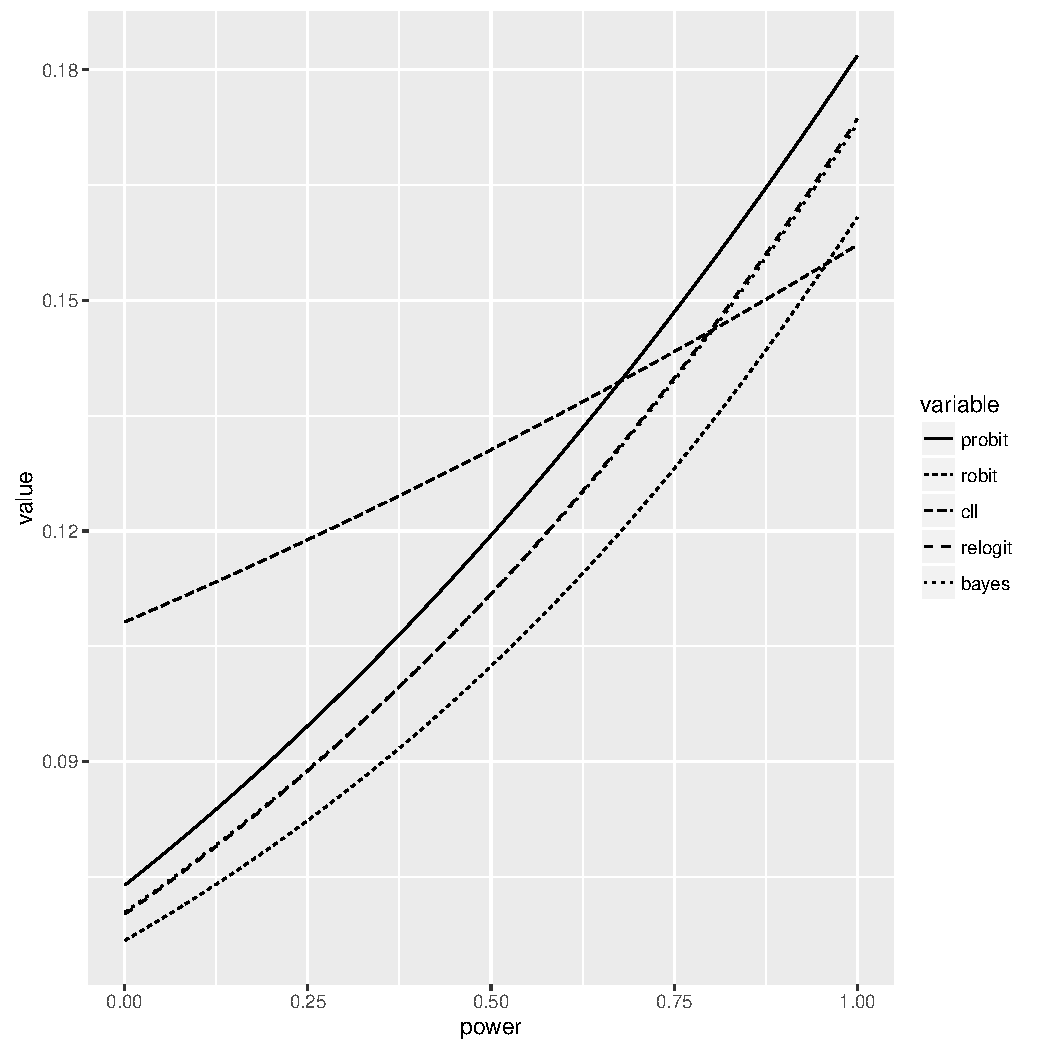
\includegraphics[width=\maxwidth]{figure/unnamed-chunk-9-1} 

\end{knitrout}

\begin{knitrout}
\definecolor{shadecolor}{rgb}{0.969, 0.969, 0.969}\color{fgcolor}\begin{kframe}
\begin{alltt}
\hlstd{pdata} \hlkwb{<-} \hlkwd{data.frame}\hlstd{(}
  \hlkwc{power} \hlstd{= mid}\hlopt{$}\hlstd{power,}
  \hlkwc{probit} \hlstd{=} \hlkwd{f_predict}\hlstd{(m_1,} \hlkwc{contig} \hlstd{=} \hlnum{0}\hlstd{,} \hlkwc{major} \hlstd{=} \hlnum{1}\hlstd{,} \hlkwc{years} \hlstd{=} \hlnum{0}\hlstd{),}
  \hlkwc{robit} \hlstd{=} \hlkwd{f_predict_robit}\hlstd{(m_2,} \hlkwc{contig} \hlstd{=} \hlnum{0}\hlstd{,} \hlkwc{major} \hlstd{=} \hlnum{1}\hlstd{,} \hlkwc{years} \hlstd{=} \hlnum{0}\hlstd{),}
  \hlkwc{cll} \hlstd{=} \hlkwd{f_predict}\hlstd{(m_3,} \hlkwc{contig} \hlstd{=} \hlnum{0}\hlstd{,} \hlkwc{major} \hlstd{=} \hlnum{1}\hlstd{,} \hlkwc{years} \hlstd{=} \hlnum{0}\hlstd{),}
  \hlkwc{relogit} \hlstd{=} \hlkwd{f_predict_zelig}\hlstd{(m_4,} \hlkwc{contig} \hlstd{=} \hlnum{0}\hlstd{,} \hlkwc{major} \hlstd{=} \hlnum{1}\hlstd{,} \hlkwc{years} \hlstd{=} \hlnum{0}\hlstd{),}
  \hlkwc{bayes} \hlstd{=} \hlkwd{f_predict}\hlstd{(m_5,} \hlkwc{contig} \hlstd{=} \hlnum{0}\hlstd{,} \hlkwc{major} \hlstd{=} \hlnum{1}\hlstd{,} \hlkwc{years} \hlstd{=} \hlnum{0}\hlstd{)}
\hlstd{)}

\hlkwd{ggplot}\hlstd{(}\hlkwc{data} \hlstd{=} \hlkwd{melt}\hlstd{(pdata,} \hlkwc{id.vars} \hlstd{=} \hlstr{"power"}\hlstd{),} \hlkwd{aes}\hlstd{(power, value))} \hlopt{+}
  \hlkwd{geom_line}\hlstd{(}\hlkwd{aes}\hlstd{(}\hlkwc{linetype} \hlstd{= variable))}
\end{alltt}
\end{kframe}
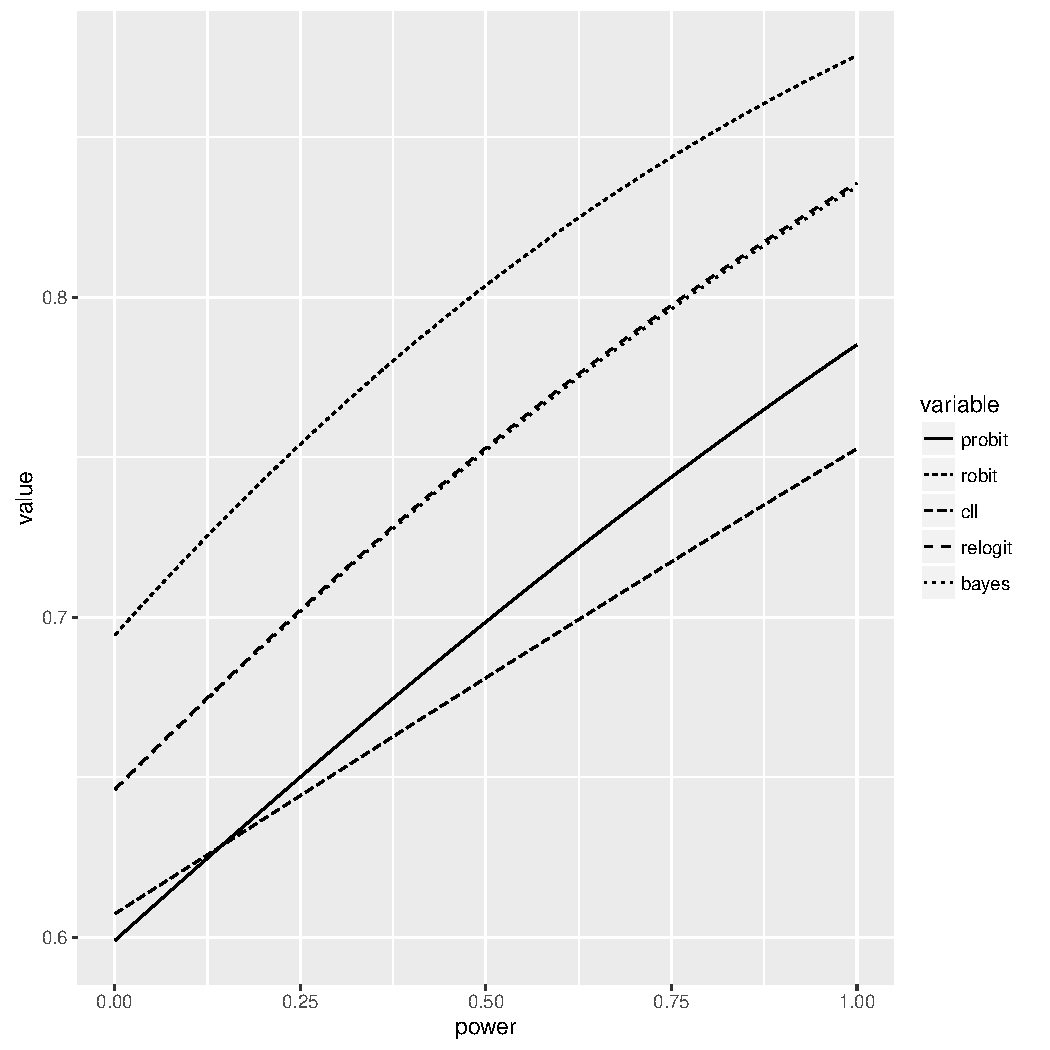
\includegraphics[width=\maxwidth]{figure/unnamed-chunk-10-1} 

\end{knitrout}


\end{document}
